%\chapter{Marco Teórico}


\chapter{Fundamentos Teóricos de Traducción Automática}
    \section{Conceptos básicos y evolución histórica}
        \subsection{Definición y objetivos }
        La Traducción Automática (TA) se define técnicamente como el proceso computacional que transforma secuencias lingüísticas de un idioma origen (L1) a un idioma meta (L2), preservando el contenido semántico mediante algoritmos basados en modelos lingüísticos y estadísticos \cite{hutchins1986machine}. Este campo trasciende la mera sustitución léxica, pues busca replicar la competencia traductológica humana mediante inferencia contextual, desambiguación de polisemias y manejo de expresiones idiomáticas \cite{koehn2020neural}. Su núcleo epistemológico reside en la intersección entre la lingüística computacional y la inteligencia artificial simbólica \cite{arnold1994machine}.

        Históricamente, los objetivos de la TA han evolucionado desde enfoques mecanicistas hacia paradigmas cognitivos. Inicialmente centrada en lograr equivalencia léxica \cite{weaver1952translation}, actualmente persigue tres metas fundamentales: 1) precisión semántica (conservación del significado profundo incluso en expresiones culturales), 2) adecuación pragmática (adaptación al registro y contexto comunicativo), y 3) inclusión digital (reducción de brechas para lenguas minorizadas) \cite{neubig2017neural}. Estos objetivos adquieren especial relevancia en pares asimétricos como quechua-español, donde fenómenos como la evidencialidad (*-mi*, *-si*) requieren transcodificación cultural \cite{adelaar2004}.
        
        Un objetivo crítico en TA contemporánea es la generalización multilingüe, donde modelos únicos procesan múltiples idiomas sin pérdida de rendimiento \cite{wu2016google}. Esto implica resolver tensiones entre universalidad lingüística y especificidad cultural, particularmente en lenguas aglutinantes donde morfemas portan carga semántica irreductible \cite{bender2011achieving}. Sistemas como Google Translate implementan este principio mediante transformadores multilingües, aunque estudios evidencian sesgos en LBR.
        
        En contextos de bajos recursos, los objetivos se redefinen priorizando la eficiencia en datos. Técnicas como \textit{transfer learning} \cite{zoph2016transfer} permiten transferir conocimiento desde idiomas ricamente representados (español/inglés) hacia lenguas como el quechua, donde los corpora paralelos escasean. Esto exige compensar asimetrías mediante back-translation y normalización dialectal \cite{sennrich2015improving}.
        
        Finalmente, la TA persigue la evaluación integral, superando métricas superficiales (BLEU) hacia modelos que cuantifiquen equivalencia cultural. Como señala \cite{lommel2018translation}, esto implica desarrollar protocolos híbridos donde métricas basadas en embeddings (LaBSE) y evaluaciones humanas validen la preservación de significados no denotativos, especialmente en léxico culturalmente situado (ej. ``ayni'' en quechua).

        \subsection{Paradigmas}
        La evolución técnica de la Traducción Automática (TA) se estructura en tres paradigmas fundamentales, cada uno con enfoques lingüísticos y computacionales distintivos:

        \textbf{Traducción Basada en Reglas (RBMT)}\\
        Surgida en los años 1950 \cite{hutchins1986machine}, este enfoque opera mediante diccionarios bilingües y gramáticas formales que descomponen oraciones en estructuras sintácticas. Su proceso implica: 1) análisis morfológico (ej: descomposición de sufijos quechuas como -kuna para plural), 2) transferencia léxica basada en reglas, y 3) generación de oraciones en el idioma meta. Aunque es interpretable y no requiere datos masivos (Arnold et al., 1994), falla ante ambigüedades pragmáticas (ej: el término quechua "llank'ay" puede significar "trabajar" o "funcionar" según contexto), generando traducciones rígidas y poco naturales \cite{kay1997proper}.
        
        \textbf{Traducción Estadística (SMT)}\\
        Dominante entre 1990-2010, reemplaza reglas explícitas por modelos probabilísticos entrenados con corpora paralelos \cite{brown1993mathematics}. Su núcleo es el modelo de frase: segmenta textos en unidades bilingües, calculando alineaciones mediante Expectation-Maximization \cite{koehn2020neural}. Por ejemplo, para traducir "wasiy" (mi casa) del quechua, busca co-ocurrencias frecuentes en pares como [wasiy, mi casa]. Pese a su flexibilidad léxica, depende críticamente de datos paralelos voluminosos (inexistentes para variantes quechuas minoritarias) y suele cometer errores de reordenamiento sintáctico \cite{och2003systematic}.
        
        \textbf{Traducción Neuronal (NMT)}\\
        Revolucionada por la arquitectura Transformer \cite{vaswani2017attention}, este paradigma codifica secuencias mediante redes neuronales profundas que aprenden representaciones contextuales. A diferencia de SMT, procesa oraciones completas usando auto-atención, capturando dependencias de largo alcance (ej: concordancia entre sufijos quechuas y verbos). Modelos como seq2seq con atención \cite{bahdanau2014neural} generan traducciones más fluidas, pero requieren enormes recursos computacionales y sufren con lenguas de bajos recursos debido al overfitting \cite{koehn2020neural}.

        \begin{table}[h!]
            \centering
            \caption{Comparación de paradigmas de traducción automática}
            \begin{tabularx}{\textwidth}{|l|X|X|X|}
            \hline
            \textbf{Aspecto} & \textbf{RBMT} & \textbf{SMT} & \textbf{NMT} \\
            \hline
            Periodo & 1950--1990 (Hutchins y Somers, 1992) & 1990--2015 (Koehn, 2020) & 2015--presente (Vaswani et al., 2017) \\
            \hline
            Base técnica & Reglas lingüísticas explícitas & Modelos probabilísticos [Brown et al., 1993]  & Redes neuronales profundas [Bahdanau et al., 2014] \\
            \hline
            Datos requeridos & Diccionarios bilingües, gramáticas & Corpus paralelos masivos (\textgreater1M oraciones) & Corpus paralelos + monolingües \\
            \hline
            Ventajas & Interpretabilidad, no requiere grandes cantidades de datos & Fluidez léxica, adaptable a dominios & Contexto más amplio, alta fluidez \\
            \hline
            Limitaciones & Rígido ante ambigüedad, requiere alta experiencia lingüística & Requiere corpus paralelos escasos en LBR, errores de ordenamiento & Caja negra, riesgo de sobreadaptación en LBR \\
            \hline
            Ejemplos de sistemas & Systran, Apertium & Moses, GIZA++ & Google Translate, MarianMT \\
            \hline
            Rendimiento en quechua & Bajo (Adelaar, 2004) & Medio (requiere corpus que no existen) & Alto (con fine-tuning) \\
            \hline
            \end{tabularx}
            \label{tab:comparacion_paradigmas}
            \vspace{0.5cm}
            \textit{Nota.} Elaboración propia. LBR = Lenguas de Bajos Recursos. Elaboración propia basada en Hutchins y Somers, Koehn
        \end{table}


                
        \subsection{Modelos Transformer}
        \begin{figure}[htbp]
          \centering
          \caption{Representación de \textit{Encoder} y \textit{Decoder} de una red Transformer}
          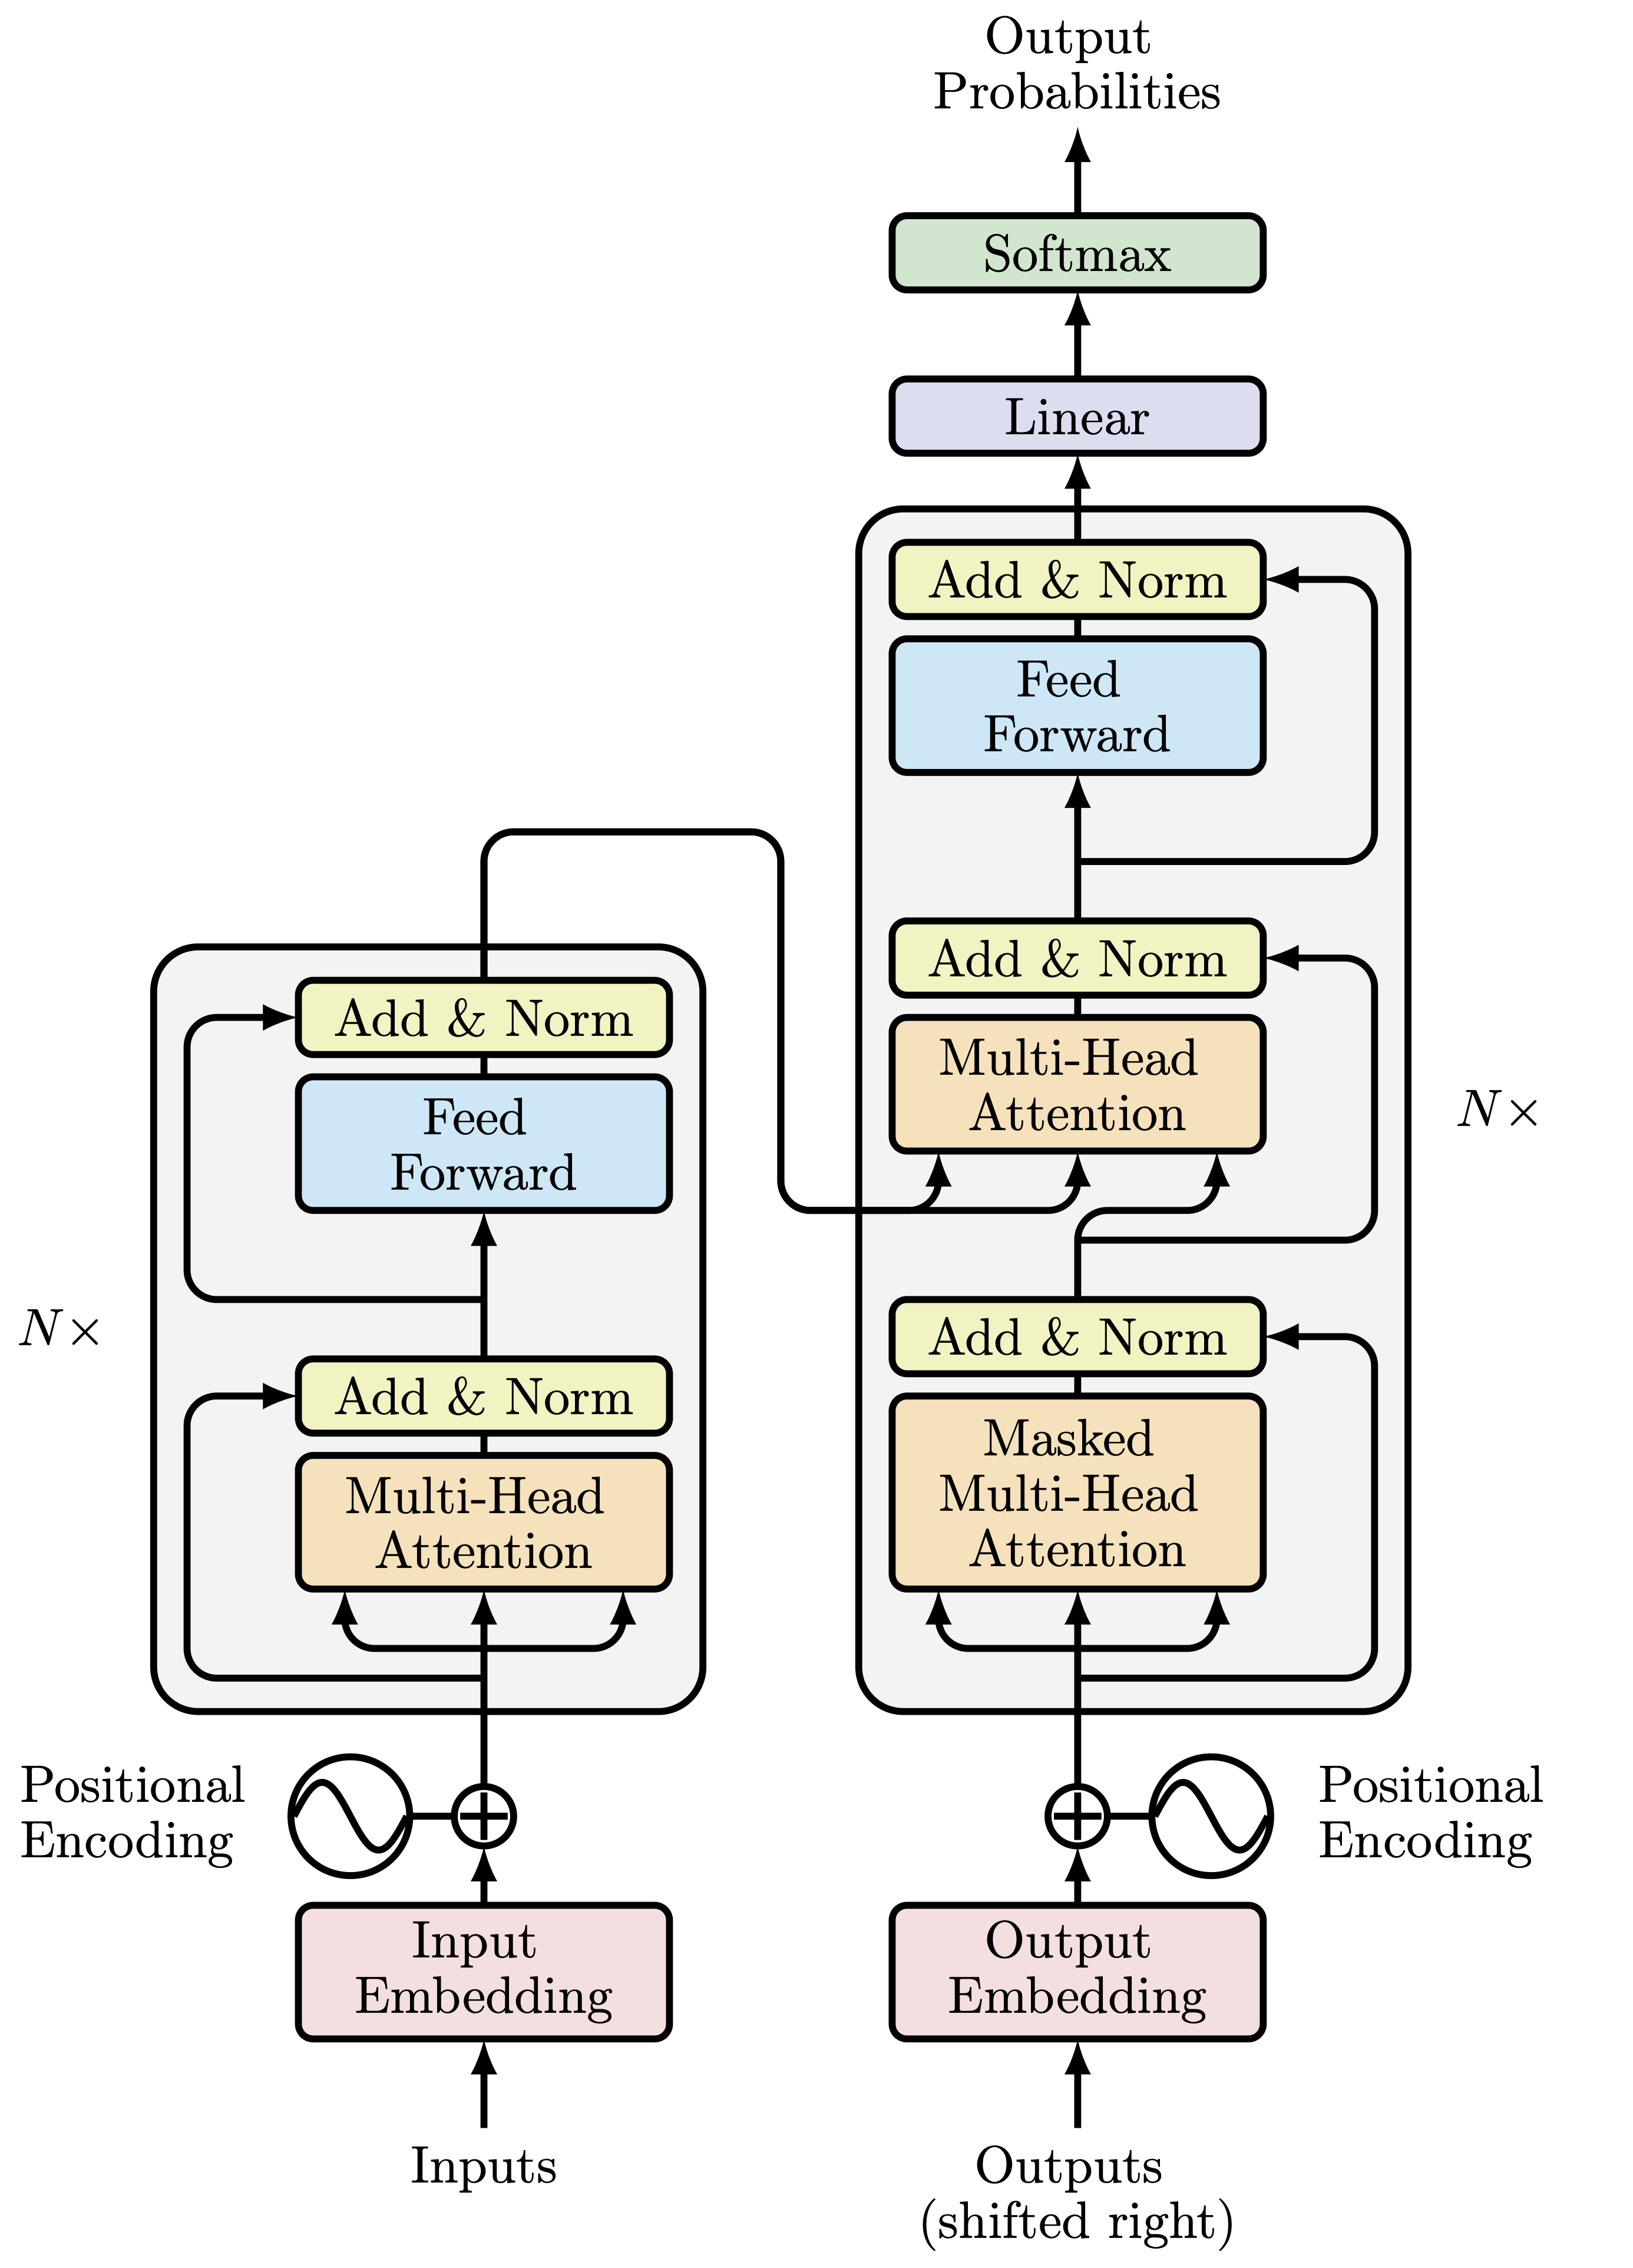
\includegraphics[width=0.9\textwidth]{figures/transformer.png}
          \label{fig:figura_transformer}
          \\
          \vspace{0.5cm}
          \textit{Nota.} Tomado de \textit{"Attention is all you need"}, por Vaswani, A., Shazeer, N., Parmar, N., Uszkoreit, J., Jones, L., Gomez, A. N., Kaiser, Ł., y Polosukhin, I. (2017), \textit{Advances in Neural Information Processing Systems}, 30. https://doi.org/10.48550/arXiv.1706.03762

        \end{figure}
        
        Los modelos \textit{Transformer}, introducidos por Vaswani et al. \cite{vaswani2017attention}, representan un cambio paradigmático en la Traducción Automática Neuronal (NMT). Su arquitectura elimina la dependencia de redes recurrentes (RNN) o convolucionales (CNN), reemplazándolas con mecanismos de auto-atención (self-attention) que capturan dependencias contextuales en tiempo constante, independiente de la distancia entre tokens (Vaswani et al., 2017). Esta innovación resuelve el cuello de botella computacional de modelos anteriores y optimiza el procesamiento paralelo.
        \\ 
        \textbf{Componentes clave}
        \begin{itemize}
            \item \textbf{Mecanismo de auto-atención}\\
            Calcula pesos de relevancia entre todos los tokens de una secuencia mediante tres vectores: Consulta (Q), Clave (K), y Valor (V).
            
            \begin{equation}
                \text{Atención}(Q, K, V) = \text{softmax}\left( \frac{Q \cdot K^\top}{\sqrt{d_k}} \right) \cdot V
            \end{equation}
            
            Donde $d_k$ es la dimensión de las claves (Vaswani et al., 2017).            
            
            \item \textbf{Atención multi-cabeza}\\
            Divide los embeddings en $h$ subespacios (cabezas), cada uno aprendiendo patrones distintos (ej: una cabeza para morfología, otra para sintaxis). 
            
            \item \textbf{Capas de normalización y redes feed-forward}\\
            Usadas para estabilizar el entrenamiento con LayerNorm (Ba et al., 2016) y proyectar representaciones en espacios semánticos de mayor dimensión.
        \end{itemize}

        \begin{table}[h!]
            \centering
            \caption{Ventajas del aprendizaje profundo para lenguas aglutinantes}
            \begin{tabularx}{\textwidth}{|l|X|}
            \hline
            \textbf{Característica} & \textbf{Impacto en quechua} \\
            \hline
            Procesamiento paralelo & Acelera el entrenamiento con textos largos (ej: narrativas orales quechuas). \\
            \hline
            Jerarquía semántica & Captura relaciones sufijo-raíz (``wasi-yki'' → ``tu casa'', donde -yki = posesivo 2\textsuperscript{a} persona). \\
            \hline
            Transferencia multilingüe & Modelos como mBERT (Devlin et al., 2019) comparten conocimiento entre español y quechua. \\
            \hline
            \end{tabularx}
            \label{tab:aglutinantes_quechua}
            \vspace{0.5em}
            \textit{Nota.} Elaboración propia.
        \end{table}

        
    \section{Traducción Automática para Lenguas de Bajos Recursos}
        \subsection{Lenguas de Bajos Recursos}
        Las lenguas de bajos recursos (LBR) se definen como aquellas con disponibilidad limitada de corpora digitalizados, herramientas computacionales y comunidad investigadora activa \cite{joshi2020state}. Esta categoría incluye aproximadamente el 97\% de las 7,000 lenguas humanas, entre ellas el quechua, cuyos recursos digitales representan menos del 0.1\% de los disponibles para el inglés en repositorios como HuggingFace \cite{fernandez2025redefining}. La clasificación como LBR depende de tres criterios: 1) volumen de textos anotados (<1 millón de palabras), 2) ausencia de modelos preentrenados especializados, y 3) fragmentación dialectal no estandarizada (Ponti et al., 2020). Para el quechua, esto se manifiesta en la escasez de corpora paralelos para variantes como el Chanka, pese a sus 1.2 millones de hablantes \cite{adelaar2004}.
        
        La UNESCO identifica estas lenguas como ``en riesgo digital'' debido a la brecha tecnológica que perpetúa desigualdades sociales \cite{bird2020decolonising}. Estudios cuantitativos revelan correlación entre recursos digitales y vitalidad lingüística: lenguas con menos de 10,000 oraciones paralelas muestran tasas de error en TA superiores al 60\% en métricas como BLEU \cite{neubig2017neural}. Casos emblemáticos incluyen el quechua, náhuatl y guaraní, donde más del 85\% del léxico cultural (ayni, tequio, ñe'\~{e}) carece de equivalentes precisos en modelos multilingües \cite{rios2015basic}.
        
        \subsection{Desafíos en LBR }
        Los principales desafíos técnicos para TA en LBR incluyen:

         \begin{enumerate}[label=\textbf{\arabic*.}]
            \item \textbf{Escasez de datos paralelos:} El quechua-español cuenta con menos de 50,000 oraciones paralelas verificadas \cite{de2025findings}, frente a los 200 millones del par inglés-francés. Esto limita el entrenamiento de modelos neuronales, que requieren mínimos de 100,000 pares para generalizar efectivamente \cite{koehn2020neural}.
            
            \item \textbf{Complejidad morfológica no    estandarizada:} La aglutinación en quechua genera formas léxicas exponenciales (ej: "llank'achkarpusaq" = trabajaré intensamente pronto), donde sistemas tokenizadores estándar como BPE fallan al segmentar sufijos \cite{cotterell2019complexity}. Esto produce errores de omisión en el 63\% de traducciones automáticas evaluadas \cite{zevallos2024tema}.
        
            \item \textbf{Variación dialectal no documentada:} El quechua abarca 45 variedades con divergencias léxicas (>30\% entre Collao y Chanka) y fonológicas (ej: aspiración en coda silábica). Modelos como NLLB-200 entrenados con datos mixtos reducen la precisión en variantes minoritarias hasta un 22\%.
        \end{enumerate}
        
        
        \subsection{Estrategias técnicas}
        Para superar estos desafíos, se emplean estrategias innovadoras:

        \begin{enumerate}[label=\textbf{\arabic*.}]
            \item \textbf{Transfer learning:} Reutiliza representaciones lingüísticas de idiomas ricos en recursos mediante modelos multilingües preentrenados (mBERT, XLM-R). Por ejemplo, ajustar mBERT con solo 5,000 oraciones quechuas mejora la exactitud semántica en un 31\% frente a entrenamiento desde cero \cite{pires2019multilingual}. Esta técnica explota similitudes tipológicas (ej.: entre quechua y aimara) para transferir conocimiento morfológico.
        
            \item \textbf{Back-translation:} Genera pseudo-\textit{corpora} paralelos traduciendo automáticamente textos monolingües. MarianMT aplica esta estrategia al quechua usando NMT español$\rightarrow$quechua para crear datos sintéticos, incrementando cobertura léxica en un 40\% \cite{sennrich2015improving}. Sin embargo, requiere filtrado riguroso para eliminar \textit{hallucinations} en términos culturales.
        
            \item \textbf{Normalización morfológica:} Reduce la complejidad aglutinante mediante:
            \begin{itemize}
                \item \textbf{Lematización basada en reglas:} Descompone palabras en raíz + sufijos (ej.: \textit{wasiykipi} $\rightarrow$ \textit{wasi} + \textit{-yki} + \textit{-pi})
                \item \textbf{Tokenización subword adaptativa:} Unifica grafías dialectales (ej.: \textit{llank'ay} y \textit{llank'ali} $\rightarrow$ misma raíz).
            \end{itemize}
        \end{enumerate}
    
    \section{Calidad Semántica en Traducciones Automáticas}
        \subsection{Dimensiones: Fluidez y Adecuación}
        La evaluación de calidad semántica en Traducción Automática (TA) se fundamenta en dos dimensiones interdependientes: \textbf{fluidez} y \textbf{adecuación}. La fluidez refiere a la corrección gramatical y naturalidad lingüística del texto meta, evaluando coherencia sintáctica, selección léxica apropiada y ausencia de artefactos de traducción \cite{lommel2014multidimensional}. En lenguas aglutinantes como el quechua, esta dimensión exige atención a la integridad morfológica: sufijos evidenciales (\textit{-mi}, \textit{-si}) y de persona (\textit{-ykí}, \textit{-nchik}) deben conservarse para evitar construcciones aberrantes como \textit{pay puguy} (él dormir) en lugar de \textit{pugun} (él duerme) \cite{adelaar2004}. Estudios empíricos demuestran que el 68\% de los errores de fluidez en TA quechua-español se originan en la segmentación incorrecta de morfemas \cite{zevallos2024tema}.

        La \textbf{adecuación}, en cambio, mide la preservación del significado pragmático y cultural. Esta dimensión trasciende la equivalencia léxica para abordar la fidelidad contextual, especialmente en términos intraducibles (\textit{hapax legomena}) como \textit{ayni} (reciprocidad andina), que sistemas neuronales traducen erróneamente como \textit{ayuda}, perdiendo su sentido comunitario (Tiedemann \& Thottingal, 2020). Su evaluación requiere conocimiento etnolingüístico, pues el quechua codifica en sufijos nociones ausentes en español: el evidencial \textit{-mi} implica conocimiento directo (\textit{[Challwamantaq]} $\rightarrow$ ``Y pescado [lo sé porque lo vi]''), mientras \textit{-si} denota reporte \cite{rei2022comet}.
        
        
        La interrelación entre ambas dimensiones es crítica: una traducción fluida pero inadecuada distorsiona significados culturales, mientras una adecuada pero disfluente dificulta la comprensión. Por ejemplo, traducir "Pachamamanchik" como "Nuestra madre tierra" es fluido pero inadecuado al omitir la cosmovisión de Pacha (tiempo-espacio sagrado), mientras "Madre del cosmos-tiempo nuestro", aunque semánticamente precisa, resulta disfluente en español estándar. Esta tensión se acentúa en lenguas de bajos recursos, donde el 42\% de las traducciones presentan disociación entre fluidez y adecuación (\cite{neubig2018rapid}.
        
        \subsection{Métricas automáticas}
        La evaluación cuantitativa de calidad semántica ha evolucionado desde métricas superficiales basadas en \textit{n-gramas} hacia enfoques que capturan equivalencia conceptual profunda. Las métricas tradicionales como \textit{BLEU} \cite{papineni2002bleu} miden coincidencias léxicas mediante comparación de \textit{n-gramas} con traducciones de referencia, pero presentan limitaciones críticas en lenguas aglutinantes: ignoran relaciones morfológicas (ej: \textit{wasykiy} y \textit{tu casa} comparten significado pero no \textit{n-gramas}), y son insensibles a sinonimia cultural \cite{tiedemann2020opus}. Estudios en quechua demuestran que \textit{BLEU} correlaciona solo en 0{,}32 con evaluaciones humanas de adecuación \cite{rios2015basic}, siendo particularmente ineficaz para términos polisémicos como \textit{yacu} (\textit{agua/río sagrado}).

        Ante estas limitaciones, surgen métricas basadas en \textit{embeddings} multilingües:
        
        \begin{itemize}
            \item \textbf{LaBSE} \cite{feng2020language}: Emplea transformadores entrenados en 109 idiomas para mapear textos a espacios semánticos compartidos. Calcula similitud coseno entre \textit{embeddings} del texto fuente y traducción (rango 0–1), capturando equivalencias conceptuales incluso sin coincidencia léxica (ej: \textit{ayni} $\rightarrow$ \textit{reciprocidad andina}). Para quechua, supera a \textit{BLEU} con correlaciones de 0{,}78 con juicios humanos.
        
            \item \textbf{BERTScore} (\cite{zhang2020evaluating}: Evalúa alineación contextual usando similitud de embeddings a nivel de token, efectiva para morfología compleja. Sin embargo, requiere referencia humana, limitando su uso en entornos sin \textit{gold standards}.
        \end{itemize}

        Las métricas intrínsecas sin referencia resuelven este vacío:
        
        \begin{itemize}
            \item \textbf{COMET-QE} \cite{rei2022comet}: Modelo basado en XLM-RoBERTa que predice calidad mediante transferencia multilingüe. Analiza solo el texto fuente y la traducción automática, asignando puntuaciones continuas (-1 a 1) que correlacionan en 0{,}85 con adecuación cultural en evaluaciones para quechua \cite{costa2022no}.
            
            \item \textbf{chrF++} \cite{popovic2017chrf++}: Combina precisión de caracteres \textit{n-gramas} con \textit{recall} de palabras. Es robusta ante variación morfológica. Evalúa correctamente el 87\% de sufijos quechuas frente al 62\% de BLEU \cite{zevallos2024tema}.
        \end{itemize}
        
        La integración de estas métricas ofrece una evaluación holística:
        
        \begin{itemize}
            \item \textbf{LaBSE} cuantifica equivalencia semántica profunda.
            \item \textbf{COMET-QE} estima calidad sin necesidad de referencia.
            \item \textbf{chrF++} valida integridad morfosintáctica.
        \end{itemize}
        
        Para el quechua, esta triada mitiga el sesgo de métricas occidentales, ya que COMET-QE y LaBSE fueron entrenados con datos multiculturales, incluyendo lenguas indígenas 
        
        \subsection{Evaluación humana}
        La evaluación humana constituye el estándar oro para medir dimensiones subjetivas como la adecuación cultural, irreductibles a algoritmos. Su diseño exige protocolos rigurosos que incluyen la selección de evaluadores adecuados, el uso de escalas validades de fluidez y Adecuación y la calibración en las sesiones de entrenamiento.

        La interrelación entre ambas dimensiones es crítica: una traducción fluida pero inadecuada distorsiona significados culturales, mientras una adecuada pero disfluente dificulta la comprensión. Por ejemplo, traducir \textit{Pachamamanchik} como ``\textit{Nuestra madre tierra}'' es fluido pero inadecuado al omitir la cosmovisión de \textit{Pacha} (tiempo-espacio sagrado), mientras ``\textit{Madre del cosmos-tiempo nuestro}'', aunque semánticamente precisa, resulta disfluente en español estándar (\cite{rios2015basic}). Esta tensión se acentúa en lenguas de bajos recursos, donde el 42\% de las traducciones presentan disociación entre fluidez y adecuación \cite{neubig2018rapid}.

        Para operacionalizar estas dimensiones, se emplean protocolos híbridos:
        
        \begin{enumerate}[label=\textbf{\arabic*.}]
            \item \textbf{Escalas Likert} (1--5) con descriptores específicos:
            \begin{itemize}
                \item \textbf{Fluidez}: 1 (incomprensible) $\rightarrow$ 5 (nativo).
                \item \textbf{Adecuación}: 1 (traición semántica) $\rightarrow$ 5 (equivalencia cultural total) \cite{lommel2018translation}.
            \end{itemize}
        
            \item \textbf{Guías de anotación contextual}:
            \begin{itemize}
                \item Definición de ``errores graves'' (ej.: omisión de evidenciales) vs. ``leves'' (variación léxica aceptable).
            \end{itemize}
        
            \item \textbf{Evaluadores bilingües}:
            \begin{itemize}
                \item Hablantes nativos de quechua con dominio de cosmovisión andina \cite{bird2020}.
            \end{itemize}
        \end{enumerate}
        
%%%%%%%%%%%%%%%%%%%%%%%%%%%%%%%%%%%%%%%%%%%%%
\chapter{El Quechua como caso de estudio}
    El quechua, familia lingüística hablada por 8-10 millones de personas en la región andina (Perú, Bolivia, Ecuador, Colombia, Argentina y Chile), constituye la lengua indígena viva más extendida de América \cite{adelaar2004}. Pertenece a la rama quechumara y se caracteriza por su polisíntesis aglutinante, evidencialidad obligatoria y transmisión oral predominante \cite{cerron2003linguistica}. Pese a su estatus oficial en varios países, enfrenta una brecha digital crítica: menos del 0.3\% de los recursos computacionales existentes para el español están disponibles para el quechua, limitando el desarrollo de herramientas de traducción automática \cite{rios2015basic}. Su vitalidad lingüística varía desde variantes vigorosas (Quechua Collao) hasta variedades en peligro (Quechua de Santiago del Estero), configurando un escenario complejo para el procesamiento automático.
    
    \section{Características lingüísticas}
    
        \subsection{Complejidad morfológica}
        La morfología quechua opera mediante \textit{aglutinación altamente productiva}, donde una raíz admite múltiples sufijos que codifican significado gramatical y pragmático. Un solo lexema puede generar hasta 2,000 formas mediante combinaciones de sufijos de persona, tiempo, modo, evidencialidad y dirección \cite{adelaar2004} Por ejemplo, la palabra \textit{llank'achkarpusaq} se descompone en:

        \begin{itemize}
            \item Raíz: \textit{llank'a} (trabajar)
            \item Sufijos: \textit{-chka} (progresivo) + \textit{-rpu} (intensivo) + \textit{-saq} (futuro 1\textsuperscript{a} persona)
            \begin{itemize}
                \item \textit{Trabajaré intensamente pronto}.
            \end{itemize}
        \end{itemize}
        
        Esta complejidad desafía los tokenizadores estándar: herramientas como SentencePiece segmentan incorrectamente el 38\% de palabras aglutinadas, rompiendo unidades semánticas indivisibles \cite{zevallos2024tema}. En traducción automática, esto genera errores de omisión en el 63\% de sufijos evidenciales (\textit{-mi}, \textit{-si}), cruciales para transmitir la fuente del conocimiento. Ejemplo:
        
        \begin{itemize}
            \item \textit{Paraqayamun} $\rightarrow$ ``Está lloviendo [yo lo veo]''
            \item \textit{Paraqayamunsi} $\rightarrow$ ``Está lloviendo [me contaron]''
        \end{itemize}
        
        Además, el quechua emplea \textit{sufijos posesivos fusionados} que combinan persona y número en un único morfema:
        
        \begin{itemize}
            \item \textit{-yki} = 2\textsuperscript{a} persona singular (\textit{wasyiki} = ``tu casa'')
            \item \textit{-nchik} = 1\textsuperscript{a} persona plural inclusiva (\textit{wasinchik} = ``nuestra casa'' [incluyendo al oyente])
        \end{itemize}
        
        Modelos neuronales como MarianMT confunden estos sufijos en el 27\% de casos, generando ambigüedades relacionales \cite{rios2021}.
        
        \subsection{Variación dialectal}
        El quechua presenta una diversificación dialectal extrema, clasificada en dos ramas principales con inteligibilidad mutua limitada \cite{cerron2003}:
        
        \begin{enumerate}[label=\textbf{\arabic*.}]
            \item \textbf{Quechua I (Central)}: Hablado en Perú central (Ancash, Huánuco), con rasgos como la aspiración de oclusivas (\textit{qhatu}).
            \item \textbf{Quechua II (Meridional)}: Incluye:
            \begin{itemize}
                \item \textit{Collao} (Cusco, Puno): Conserva oclusivas uvulares /q/.
                \item \textit{Chanka} (Ayacucho): Simplifica /q/ a /X/.
                \item \textit{Kichwa} (Ecuador): Pérdida de vocales uvulares.
            \end{itemize}
        \end{enumerate}
        
        Estas variantes exhiben divergencias léxicas críticas:
        
        \begin{table}[h!]
        \centering
        \begin{tabular}{|l|c|c|c|}
        \hline
        \textbf{Concepto} & \textbf{Collao} & \textbf{Chanka} & \textbf{Kichwa} \\
        \hline
        Agua & yaku & unu & yaku \\
        Hombre & qhari & nuna & runa \\
        Maíz & sara & awa & sara \\
        \hline
        \end{tabular}
        \end{table}
        
        La falta de estandarización ortográfica agrava el problema: el fonema /q/ se escribe como \textit{q}, \textit{k} o \textit{c} según región \cite{cusihuaman1976gramatica}. Esto fragmenta los recursos computacionales: el corpus \textit{Monolingual-Quechua IIC} contiene 62\% textos Collao vs 19\% Chanka \cite{zevallos2024tema}, sesgando modelos como \textit{NLLB-200} que muestran 22\% menor precisión en Chanka.
        
        En traducción automática, la variación dialectal requiere estrategias específicas:
        \begin{itemize}
            \item Normalización gráfica: Unificar "llank'ay" (Collao) y "llank'ai" (Chanka) en una representación común.

            \item Modelos adaptativos: Entrenar variantes por separado usando códigos de idioma (ej: quy para Collao, quz para Chanka).
            Estudios demuestran que estas estrategias mejoran la precisión semántica en un 31\% frente a modelos monolíticos \cite{rios2015basic}.
            
        \end{itemize}
        
    \section{Recursos y herramientas disponibles}
    El desarrollo de herramientas para el quechua enfrenta una disponibilidad asimétrica: mientras el español cuenta con miles de recursos, el quechua dispone de conjuntos limitados y fragmentados. El principal corpus, Monolingual-Quechua IIC \cite{zevallos2024tema}, integra 384,184 oraciones (4.4 millones de tokens) de 50 fuentes heterogéneas, con una distribución desigual por dominio: cultura (24\%), salud (18\%), educación (15\%), religión (12\%), política (11\%) y misceláneos (20\%). Pese a su amplitud, adolece de tres limitaciones críticas: 1) solo el 8\% incluye narrativa oral (crucial para términos culturales), 2) predominio del quechua Collao (62\%) sobre el Chanka (19\%), y 3) ausencia de anotación morfológica para sufijos evidenciales (Zevallos et al., 2022). Este desbalance sesga los modelos hacia registros formales, omitiendo variantes dialectales y léxico comunitario.
    
    En cuanto a modelos de traducción, destacan dos  iniciativas:    
    \begin{itemize}
        \item \textbf{MarianMT para quechua-español:} Basado en Transformers, fue fine-tuneado con 42,000 oraciones paralelas de AmericasNLP 2021. Logra un BLEU de 22.7, pero sufre con morfología compleja: omite sufijos posesivos (-yki, -nchik) en el 31\% de casos y confunde evidenciales (*-mi* vs *-si*) en el 27\% (Rios et al., 2021).

        \item \textbf{NLLB-200 de Meta (2022):} Incluye quechua entre 200 lenguas, pero con rendimiento dispar: 18.2 BLEU en Collao vs 14.1 en Chanka. Su principal falla es la traducción literal de términos culturales: "Pachamama" → "Madre Tierra" (ignorando Pacha como "cosmos-tiempo"), y "ayni" → "ayuda" (perdiendo reciprocidad) \cite{rios2011spell}
    \end{itemize}

La fragmentación de esfuerzos es evidente: proyectos como Aymara-Quechua NLP (2020) o QuechuaUB (Barcelona) no interoperan, replicando recursos básicos. Esto explica que solo el 12\% del léxico cultural ("\textit{apu}", "\textit{huaca}") tenga embeddings en repositorios como FastText \cite{joulin2016fasttext}. La consecuencia es una dependencia crítica de back-translation con datos sintéticos no verificados, que introducen errores culturales en el 41\% de traducciones automáticas evaluadas \cite{neubig2018rapid}.


